\chapter{Motivating Scenario}
\label{chap:motivatingScenario}

In order to help in understanding the concepts of organizational modeling, the below motivating scenario has been taken and explained through the notations mentioned in Section \ref{sec:resourcecentricorganizationalmodeling}. This scenario also helps in validating the developed web editor in Chapter \ref{chap:casestudy}. The motivating scenario has been chosen based on the collected real life scenarios provided in the thesis work \cite{Sierr2015}. The scenario of this example was taken from the context of manufacturing sector. The main intention of the organization in this scenario is \textit{to increase the quarterly revenue and number of unit sales}. In order to achieve this main intention through our organizational modeling approach, as a first step we need to break the intention from abstract level into concrete levels like strategies, sub-intentions, process definitions, resource definitions etc. This intention can be achieved by following all of the below mentioned strategies, which requires resources with matching capabilities.  
\begin{enumerate}
	\item Increasing the revenue through expanding the market sales. 
	\item Through improving the excellence of the product which in turn brings back old and new customers.
	\item Through increasing the advertisement which helps in customer knowing about the product.
\end{enumerate}

In this chapter, the first section provides an overview about the motivating scenario followed by second section that explains in detail about the motivating scenario. The third section provides an abstract overview about the entity types in the motivating scenario which will be explained in a concrete way, in the following Chapter \ref{chap:casestudy}.

%%%%%%%%%%%%%%%%%%%%%%%%%%%%%%%%%%%%%%%%%%%%%%%%%%%%%%%%%%%%%%%%%%%%%%%%%
\section{Overview of Motivating Scenario}
\label{sec:overview}
%%%%%%%%%%%%%%%%%%%%%%%%%%%%%%%%%%%%%%%%%%%%%%%%%%%%%%%%%%%%%%%%%%%%%%%%%
The motivating scenario provided in this chapter serves as a running example throughout this document, to help the reader in understanding the concepts better. We have taken a scenario of laptop manufacturing company, where the \textit{main intention} of the organization in current context is to increase the revenue of the company. The participating resources work towards one \textit{main intention} and certain \textit{sub-intentions}. Sub-intentions are part of main intention, which helps the resources to modularize and achieve the main intention. Also each sub-intention has certain type of relationship with main-intention. For example in our below described motivating scenario in Section \ref{sec:scenario} one of the sub-intention is to \textit{expand sales geographically} . Before executing this sub-intention, few ground works like collection of laptop usage statistics such as average buying capacity of the consumers, average computer knowledge in the new area has to be done. Thus the execution of main intention i.e \textit{increase revenue and number of unit sales}, requires collaboration of people with different skills and expertise. People who has skills to collect and study statistics can serve as external resources. As new intentions may emerge dynamically the team working towards the achievement of main intention should also be ready to accommodate new resources with new capabilities and skills. There is also a software development team, which work towards achievement of one of the sub-intention \textit{improve help desk}, i.e this team develops software that automatically attends and records user queries.  The management of the project is done through the support of project management software called Redmine \footnote{http://www.redmine.org/}. The participating human resources are members of business oriented social network called XING \footnote{http://www.xing.com/}.
 


%%%%%%%%%%%%%%%%%%%%%%%%%%%%%%%%%%%%%%%%%%%%%%%%%%%%%%%%%%%%%%%%%%%%%%%%%
\section{Resource-centric Organizational Modeling Example}
\label{sec:scenario}
%%%%%%%%%%%%%%%%%%%%%%%%%%%%%%%%%%%%%%%%%%%%%%%%%%%%%%%%%%%%%%%%%%%%%%%%%
 The concept of resource centric organizational modeling can be explained with the following scenario in a manufacturing organization. ABC Ltd. is a budding computer technology company which designs, develops, manufactures and sells personal computers, tablets and laptops. The CEO's intention of the quarter is to increase the revenue and number of unit sales. The initial context describes the situation before starting the execution of intention. The initial context also provides description that motivates to start the process. The final context describes the situation that is achieved once the intention executed successfully. Intentions connect initial context definitions with final context definitions \cite{Sungur2014a}. The sub-intentions are the intermediate intentions which describes the expected outcome in a measurable form. Intentions reach strategy implementations through achieving strategies which are plans of action designed to meet a specific intention. 

 The example scenario ABC Ltd. follows top-down approach of organizational modeling i.e., how organization's higher level intentions can be achieved by amalgamation of specific, measurable and realistic sub-intentions, strategies etc. The whole view has been divided into Intention view and Strategy view. The \textit{Intention View} shown in the Figure\ref{fig:motivatingscenario} provides only the details of intention and its associated strategies. There can be multiple strategies followed to achieve an intention. The \textit{Strategy View} shown in the Figure\ref{fig:motivatingscenario} connects big picture of each strategy with individual intentions that has to be carried out. In this type of process modeling, strategies are self-contained and loosely coupled. This is the reason when we extract only the strategies from Organizational Process Modeling it would be similar to Informal Process Essential Modeling. 
 
 \begin{figure}
 	\centering
 	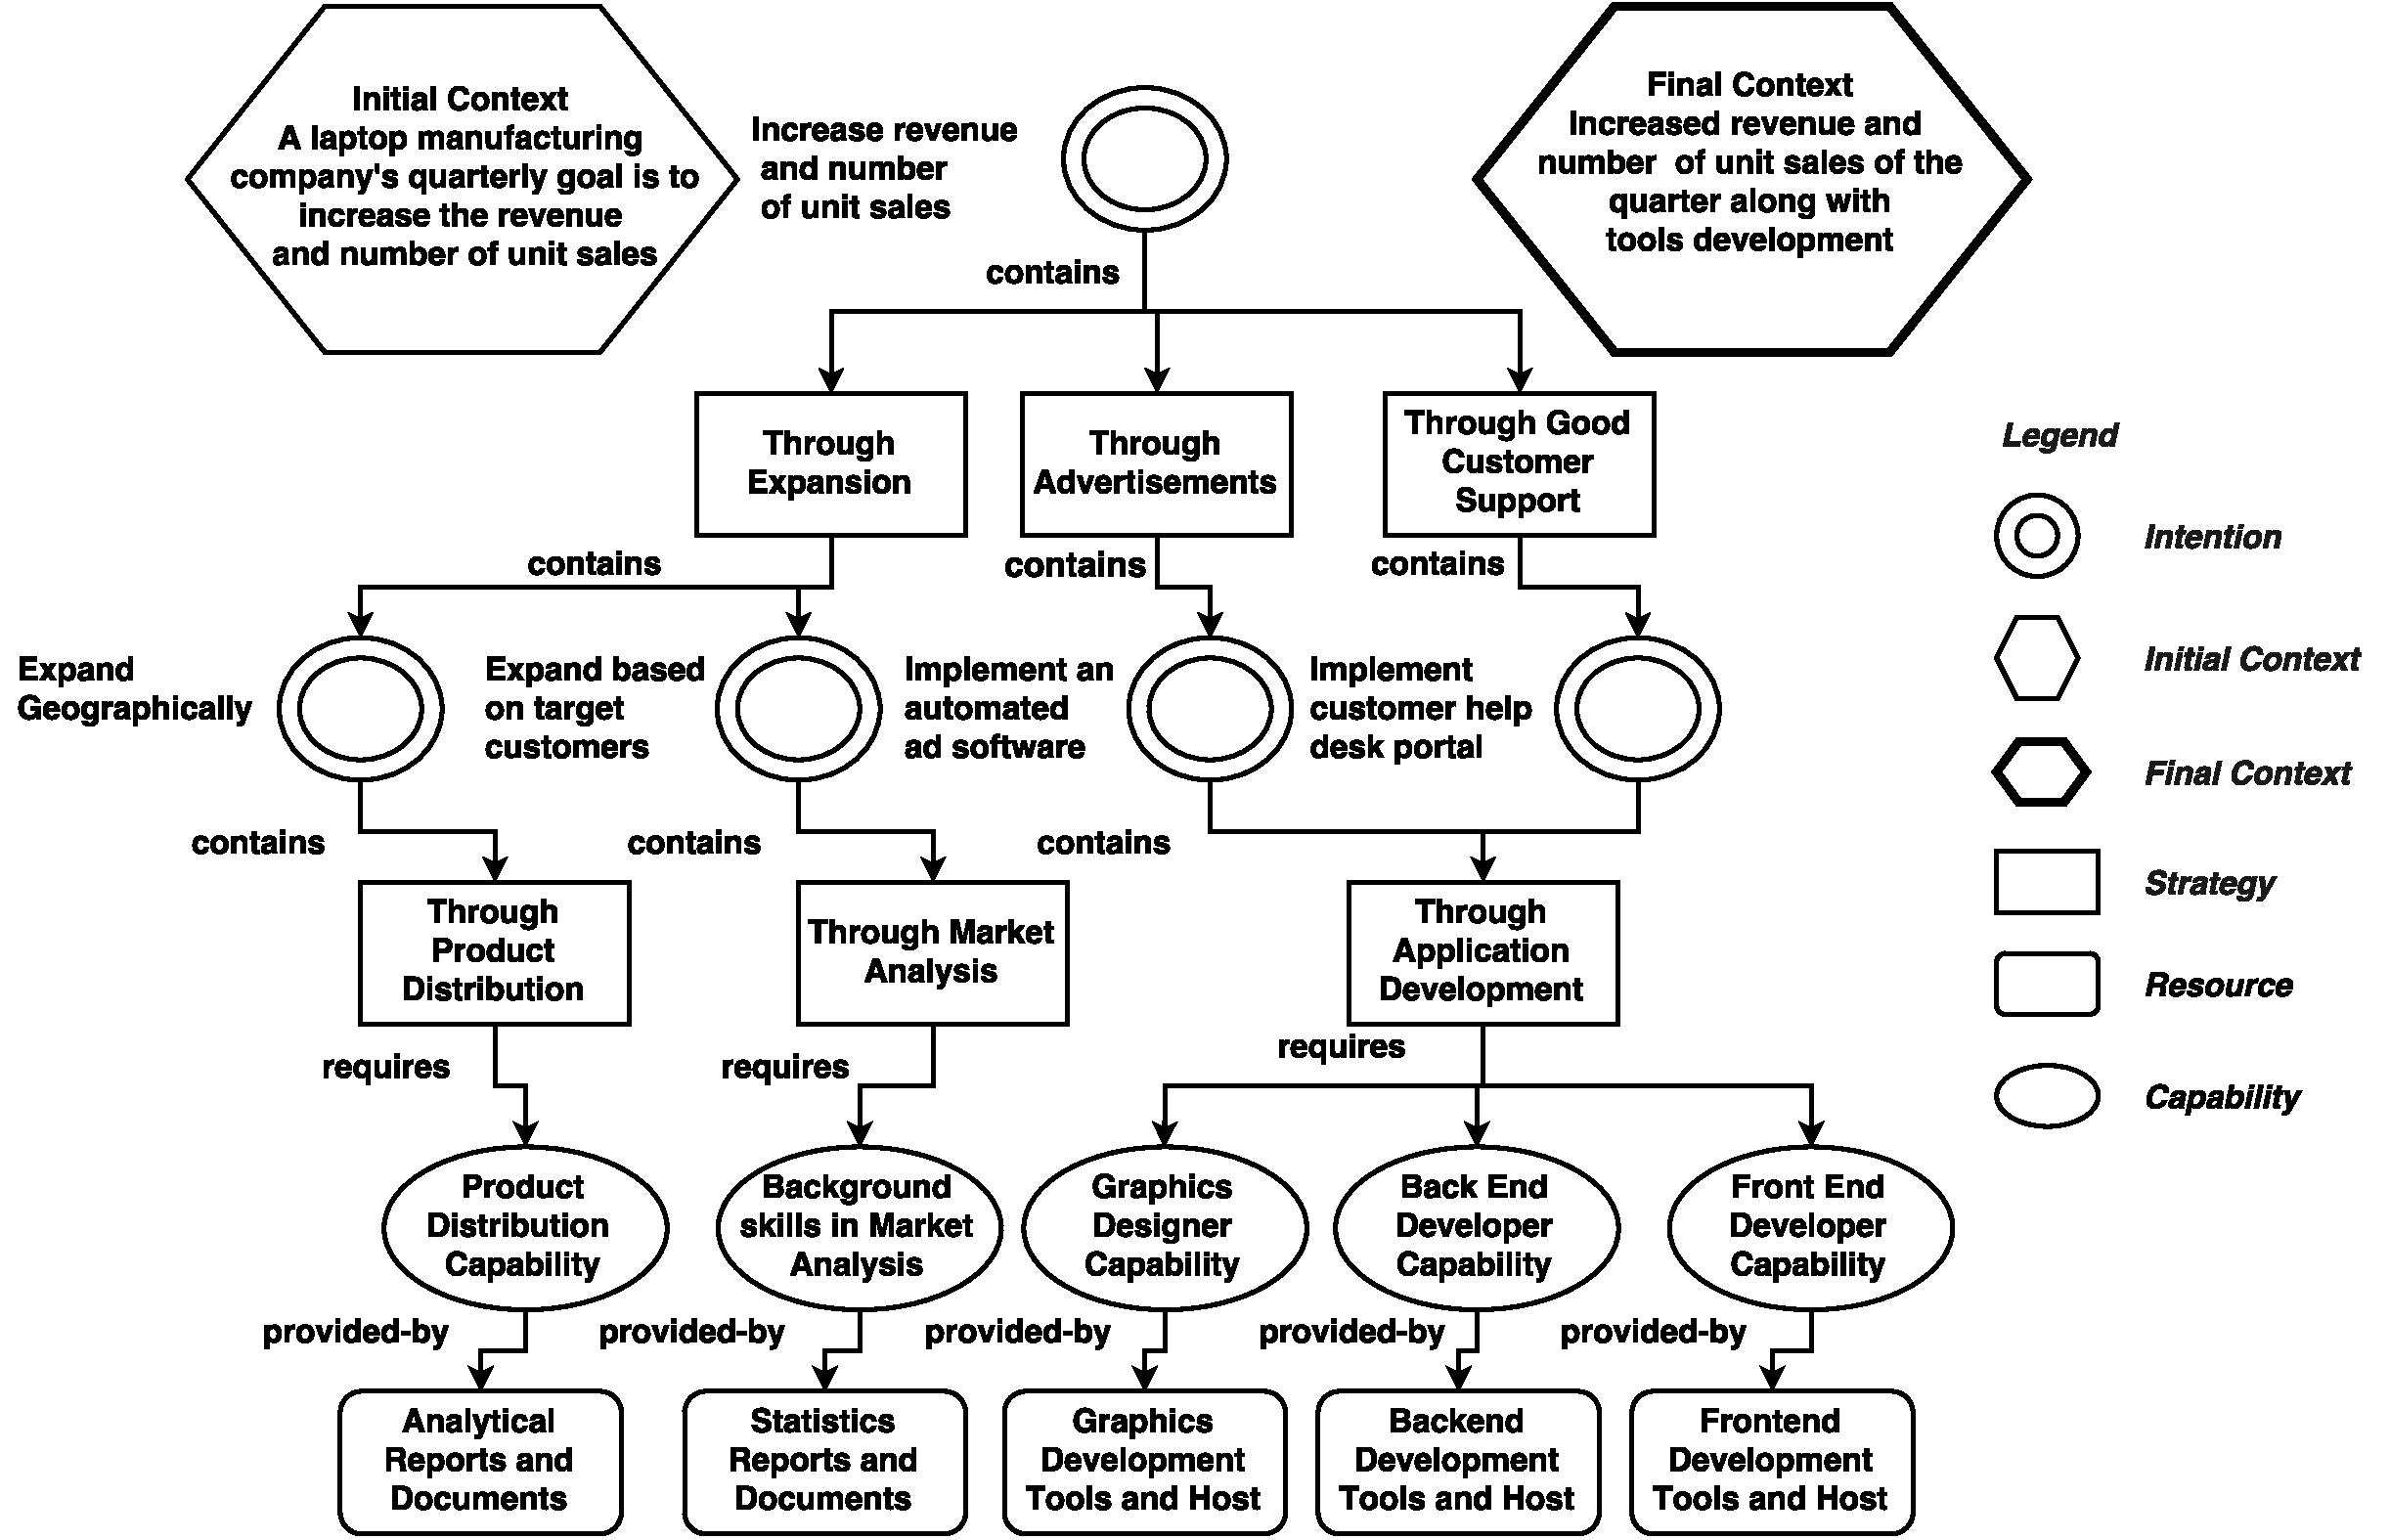
\includegraphics[width=\textwidth]{MotivatingScenario.pdf}
 	\caption{Motivating Scenario}
 	\label{fig:motivatingscenario}
 \end{figure}

 The Strategy view  in the Figure\ref{fig:motivatingscenario} depicts big picture of each strategy. Strategies are associated with both intentions and capabilities. Capabilities are related to resources. As each intention needs certain capability to successfully execute the intention they both are connected using the verb \textit{"requires"}. Resources are the potential holder of the capability i.e., to satisfy a capability we need resources. The capability and its associated resources are linked using the verb \textit{"satisfied-by"}. 






%%%%%%%%%%%%%%%%%%%%%%%%%%%%%%%%%%%%%%%%%%%%%%%%%%%%%%%%%%%%%%%%%%%%%%%%%
\section{An Abstract View of Entity Types}
\label{sec:entities}
%%%%%%%%%%%%%%%%%%%%%%%%%%%%%%%%%%%%%%%%%%%%%%%%%%%%%%%%%%%%%%%%%%%%%%%%%
 --- This section discusses in details, about each entity types of the motivating scenario and 
 their images---
 

%%%%%%%%%%%%%%%%%%%%%%%%%%%%%%%%%%%%%%%%%%%%%%%%%%%%%%%%%%%%%%%%%%%%%%%%%
\subsection{Organizational Intentions} 
\label{sec:intentions}
%%%%%%%%%%%%%%%%%%%%%%%%%%%%%%%%%%%%%%%%%%%%%%%%%%%%%%%%%%%%%%%%%%%%%%%%%
Intentions can contradict themselves, for example in our motivating scenario IT system managers are not willing to give up the systems they are working for a long time even if it is a better solution for organization as whole . This real life example scenario has been provided in the thesis work \cite{Sierr2015} and also it has been suggested that such contradicting intentions has to be handled in some way. Thus our developed web editor has also provision to add both sub-intentions and contradicting intentions for any intention.  


%%%%%%%%%%%%%%%%%%%%%%%%%%%%%%%%%%%%%%%%%%%%%%%%%%%%%%%%%%%%%%%%%%%%%%%%%
\subsection{Organizational Strategies} 
\label{sec:strategies}
%%%%%%%%%%%%%%%%%%%%%%%%%%%%%%%%%%%%%%%%%%%%%%%%%%%%%%%%%%%%%%%%%%%%%%%%%
Strategies are used to identify the most appropriate method of utilizing the capabilities. 


%%%%%%%%%%%%%%%%%%%%%%%%%%%%%%%%%%%%%%%%%%%%%%%%%%%%%%%%%%%%%%%%%%%%%%%%%
\subsection{Organizational Capabilities}
\label{sec:capabilities}
%%%%%%%%%%%%%%%%%%%%%%%%%%%%%%%%%%%%%%%%%%%%%%%%%%%%%%%%%%%%%%%%%%%%%%%%%
Describing  capabilities as \textit{ability to do something}, suggests that capabilities are related to intentions. Resources tends to posses certain capabilities that allow them to do something that they want or need to do something. 



%%%%%%%%%%%%%%%%%%%%%%%%%%%%%%%%%%%%%%%%%%%%%%%%%%%%%%%%%%%%%%%%%%%%%%%%%
\subsection{Organizational Resources} 
\label{sec:resources}
%%%%%%%%%%%%%%%%%%%%%%%%%%%%%%%%%%%%%%%%%%%%%%%%%%%%%%%%%%%%%%%%%%%%%%%%%

Each resources has different types of relationship with other resources based on how they communicate with other resources \cite{Sungur2015}. For example in our motivating scenario described in Section \ref{sec:scenario} has one of the sub-intention as \textit{through excellence}. This sub-intention can be achieved by providing skills improvement training to the employees or by recuriting newly skilled employee. Here the manager has permissions to decide whether to improve skills of existing employee or recruit new employee. But the team lead has restricted permission like what type of skills are required for the project based on decision of manager. The Informal Process Essentials (IPE) approach proposed by Sungur et al. \cite{Sungur2015}, paves the way to create models with definitions of key actors e.g manager, team lead and definitions of suppoting resources such as Mediawiki \footnote{http://www.mediawiki.org/}.

A \textit{resource organizer} is responsible for gathering definitions about the resources which are required by business experts for modeling \cite{Sungur2014a}.  



%%%%%%%%%%%%%%%%%%%%%%%%%%%%%%%%%%%%%%%%%%%%%%%%%%%%%%%%%%%%%%%%%%%%%%%%%
\subsection{Organizational Processes} 
\label{sec:processes}
%%%%%%%%%%%%%%%%%%%%%%%%%%%%%%%%%%%%%%%%%%%%%%%%%%%%%%%%%%%%%%%%%%%%%%%%%

%%%%%%%%%%%%%%%%%%%%%%%%%%%%%%%%%%%%%%%%%%%%%%%%%%%%%%%%%%%%%%%%%%%%%%%%%
\subsection{Informal Process Instances} 
\label{sec:ipinstances}
%%%%%%%%%%%%%%%%%%%%%%%%%%%%%%%%%%%%%%%%%%%%%%%%%%%%%%%%%%%%%%%%%%%%%%%%%